\documentclass[10pt,a4paper,openany,notitlepage]{article}
\usepackage[latin1]{inputenc}
%\usepackage[italian]{babel}
\usepackage{hyperref}
\hypersetup{
    colorlinks,
    citecolor=gray,
    filecolor=red,
    linkcolor=blue,
    urlcolor=blue
}
\usepackage{amsmath}
\usepackage{geometry}
%\usepackage{xcolors}
\usepackage{graphicx}
\usepackage{pdflscape}
%\usepackage{lscape}
\usepackage{amsfonts}
\usepackage{amssymb}
\usepackage{listings}
\lstset{%
	commentstyle=\color{green},
	frame=single,
	keepspaces=true,
	keywordstyle=\color{blue},
	numbers=left,
	numberstyle=\tiny\color{black},
	rulecolor=\color{black},
	columns=flexibile
        basicstyle=\ttfamily
}
\author{Davide Polonio (1070162), Alessandro Bari(1074356)}
\title{Progetto di Basi di Dati 2015}
\begin{document}
\maketitle
\newpage
\tableofcontents
\newpage

\section{Progettazione Concettuale}

\subsection{Studio di fattibilit\`a} 

\paragraph*{Priorit\`a di realizzazione}
Come priorit\`a di realizzazione abbiamo deciso di implementare le seguenti feature:
\begin{itemize}
\item Percentuale di sconto basata sul numero di acquisti effettuato da un acquirente iscritto al servizio.
\item Gestione degli ordini e delle fatture del negozio, oltre che degli scontrini e delle vendite effettuate riferite agli iscritti.
\item Gestione e organizzazione dei turni per i dipendenti.
  \item Catalogazione prodotti in diverse categorie (a cui appartengono diverse percentuali di sconto).
\end{itemize}

\subsection{Raccolta e analisi dei requisiti}

\subsubsection{Analisi dei requisiti}
Per i clienti \textbf{iscritti} identificati da un codice, vogliamo tenere conto dell'identit\`a e dei suoi acquisti effettuati.



Ogni \textbf{prodotto} \`e identificato da un codice, vogliamo tenere conto delle informazioni base e della quantit\`a disponibile e catalogarlo in una delle cinque \textbf{categorie}, identificate come: porcellane, pentolame, liste nozze, stoffe, stoviglie.


Ad ogni categoria sono associati possibili \textbf{sconti} in base ad una distribuzione per livelli e con una relativa percentuale.


I \textbf{dipendenti}, responsabili ognuno di una singola categoria, sono identificati da un codice e sono organizzati per turni.


Vogliamo tener conto degli ordini di merce ai \textbf{fornitori} con rispettive \textbf{fatture}. \\


\subsubsection{Glossario dei termini}
\begin{center}
\begin{tabular}{ l | p{5cm} | p{3cm} | p{3cm} }
%\hline

\textbf{Termine} & \textbf{Descrizione} & \textbf{Sinonimi} & \textbf{Collegamenti} \\ \hline

Iscritto & Compratore abituale iscritto a questa lista per avere diritto a sconti speciali. Pu\`o essere un dipendente. & Cliente abituale & Acquisto, Scontrino \\ \hline

Scontrino & Scontrino attestante lo storico degli acquisti. & Storico, acquisto & Iscritto, Prodotto \\ \hline

Categoria & Cinque insiemi di prodotti. Un prodotto pu\`o appartenere ad un'unica categoria. Ogni categoria ha il suo univoco responsabile. & & Sconto, Dipende, Prodotto. \\ \hline

Sconto & Spetta solamente al cliente iscritto. Per ogni categoria esistono diversi livelli in base agli acquisti, a cui corrisponde una percentuale di sconto. & & Categoria. \\ \hline

Dipendente & Responsabile di una singola categoria. Pu\`o essere un cliente ma non un fornitore. & Responsabile & Categoria \\ \hline

Prodotto & Ogni prodotto pu\`o appartenere ad una sola categoria. & Oggetti, Prodotto ordinati o acquistati & Categoria, Fattura, Scontrino \\ \hline

Fattura & Pi\`u unit\`a di prodotto possono essere ordinate a fornitori diversi. Modifica il campo quantit\`a disponibile di prodotto. & Ordine & Fornitore, Prodotto \\ \hline

Fornitore & Forniscono i prodotti attraverso gli ordini. Un fornitore non pu\`o essere un cliente e pu\`o fornire prodotti di diverse categorie & & Ordine \\


%\hline
\end{tabular}
\end{center}


\subsubsection{Schema Concettuale}

\paragraph*{Lista delle Entit\`a}

\begin{itemize}

\item \underline{Dipendente}: lista dei dipendenti del negozio.
  
  \begin{itemize}

  \item Codice dipendente (PK)
    
  \item Informazioni: dati anagrafici e di recapito del dipendente
    \begin{itemize}
    \item Nome
    \item Cognome
    \item Data di nascita
    \item Codice Fiscale
    \item Telefono
    \item E-mail
    \end{itemize}
    
  \item Indirizzo:
    \begin{itemize}
    \item Via
    \item Numero
    \item Citt\`a
    \end{itemize}

  \end{itemize}

\item \underline{Categoria}: insieme di prodotti
  \begin{itemize}
  \item Nome Categoria (PK)
  \item Responsabile (FK)
  \end{itemize}

\item \underline{Sconto}: entit\`a destinata a contenere tutti i gradi di sconto di tutte le categorie
  \begin{itemize}
  \item Livelli (PK)
  \item Categorie (FK)
  \item Tetto Max
  \end{itemize}

\item \underline{Prodotto}: lista di tutti i prodotti in vendita
  \begin{itemize}
  \item Codice Prodotto (PK)
  \item Quantit\`a
  \item Percentruale iva
  \item Categoria (FK)
  \end{itemize}

\item \underline{Specifica}: descrizione base sul prodotto
  \begin{itemize}
  \item Codice Prodotto (FK)
  \item Descrizione
  \item Nome
  \item Foto
  \end{itemize}

\item \underline{Fattura}: contenente tutti gli attestati di avvenuto ordine per un certo numero di prodotti
  \begin{itemize}
  \item Codice Fattura (PK)
  \item Codice Prodotto (FK)
  \item Quantit\`a
  \item Data
  \item Fornitore (FK)
  \end{itemize}

\item \underline{Fornitore}: lista di tutti i venditori da cui il negozio acquista i prodotti
  \begin{itemize}
  \item Nome (PK)
  \item Contatto
    \begin{itemize}
    \item Fax
    \item Telefono
    \item E-mail
    \end{itemize}

  \item Indirizzo:
    \begin{itemize}
    \item Via
    \item Provincia
    \item Citt\`a
    \end{itemize}
  \end{itemize}
  Di cui sono presenti le seguienti generalizzazioni:
  \begin{itemize}
  \item \underline{Artigiano}: Fornisce prodotti fatti a mano
  \item \underline{Grossista}: Fornisce prodotti all'ingrosso
  \end{itemize}

\item \underline{Scontrino}: registro di tutti le vendite effettuate ai clienti iscritti
  \begin{itemize}
  \item Codice Scontrino (PK)
  \item Data (PK)
  \item Quantit\`a
  \item Codice Prodotto (FK)
  \end{itemize}

\item \underline{Cliente}: lista dei clienti, di cui abbiamo creato la seguente generalizzazione parziale:
  \begin{itemize}
  \item \underline{Iscritto}: clienti iscritti
    \begin{itemize}
    \item Codice Iscritto (PK)
    \item Indirizzo:
      \begin{itemize}
      \item Via
      \item Provincia
      \item Citt\`a
      \end{itemize}

    \item Contatto
      \begin{itemize}
      \item Fax
      \item Telefono
      \item E-mail
      \end{itemize}

    \item Identit\`a
      \begin{itemize}
      \item Nome
      \item Cognome
      \end{itemize}

    \end{itemize}
  \end{itemize}
  
\end{itemize}


\subsubsection{Lista delle Relazioni}

\begin{itemize}

\item \underline{Responsabile}: relazione tra Dipendente-Categoria.
  \begin{itemize}
  \item Presenza di due attributi:
  \begin{itemize}
  \item Turno
  \item Data di inizio
  \end{itemize}
  La cardinalit\`a \`e (1,1) in quanto ogni dipendente \`e responsabile solamente di una categoria e vi lavora in una determinata data e in un rispettivo turno.

  \end{itemize}

\item \underline{Scaglioni}: relazione tra Categoria-Sconto. \`E una cardinalit\`a (0,N) da Categoria $\to$ Sconto, mentre la cardinalit\`a risulta essere (1,N) da Sconto $\to$ Categoria. \newline
Ogni Categoria presenta dei diversi scaglioni di sconti in base al livello di acquisto.

\item \underline{Appartenenza}: relazione tra Categoria-Prodotto. Da Prodotto $\to$ Categoria abbiamo imposto una cardinalit\`a di tipo (1,1) in quanto un Prodotto deve appartenere a una ed una sola Categoria. \newline
  La cardinalit\`a \`e (0,N) da Categoria $\to$ Prodotto in quanto una nuova categoria pu\`o non contenere prodotti.\newline
  Si prenda l'esempio della Categoria \textit{Liste Nozze}: quando il negozio non sta svolgendo nessuna attivit\`a per matrimoni la categoria \textit{Lista Nozze} risulter\`a essere vuota. %DA FARE FRAMEBOX PERCHÈ ESEMPIO

\item \underline{Definito}: relazione tra Prodotto-Specifica. La cardinalit\`a tra Prodotto e Specifica \`e (1,1) in quanto ogni prodotto ha una singola specifica.

\item \underline{Registrato}: relazione tra Fattura-Prodotto. Da Prodotto $\to$ Fattura abbiamo una relazione di tipo (1,N) in quanto un prodotto deve risultare registrato in una fattura. \newline
  Da Fattura $\to$ Prodotto la cardinalit\`a \`e (1,N) perch\`e una fattura per essere emessa deve contenere uno o pi\`u prodotti

\item \underline{Emesso}: relazione tra Fattura-Fornitore. Da fattura a fornitore la cardinalit\`a \`e (1,1): una fattura pu\`o essere solamente emessa da un singolo fornitore. \newline
  Da Fornitore $\to$ a Fattura \`e (1,N) in quanto viene memorizzato solamente un fornitore che abbia almeno emesso una o pi\`u fatture al negozio.

\item \underline{Certifica}: relazione tra Prodotto-Scontrino. Ha cardinalit\`a (0,N) in Prodotto $\to$ Scontrino siccome un prodotto pu\`o esser stato acquistato da zero a pi\`u volte, invece da Scontrino $\to$ Prodotto vi \`e una cardinalit\`a (1,N), uno scontrino infatti certifica almeno un prodotto.

\item \underline{Ottiene}: relazione tra Scontrino-Cliente. In Scontrino $\to$ Cliente vi \`e una relazione (1,1) in quanto uno scontrino si riferisce ad un singolo acquirente, mentre tra Cliente $\to$ Scontrino vi \`e una relazione (1,N) ne consegue che un cliente pu\`o fare molti acquisti. Un cliente per essere definito tale deve almeno aver compiuto un acquisto.
  
\end{itemize}

%Passi successivi: Schema, Progettazione logica, Schema Normalizzato.

\newpage
\subsection{Schema E-R}

\begin{figure}[h!]
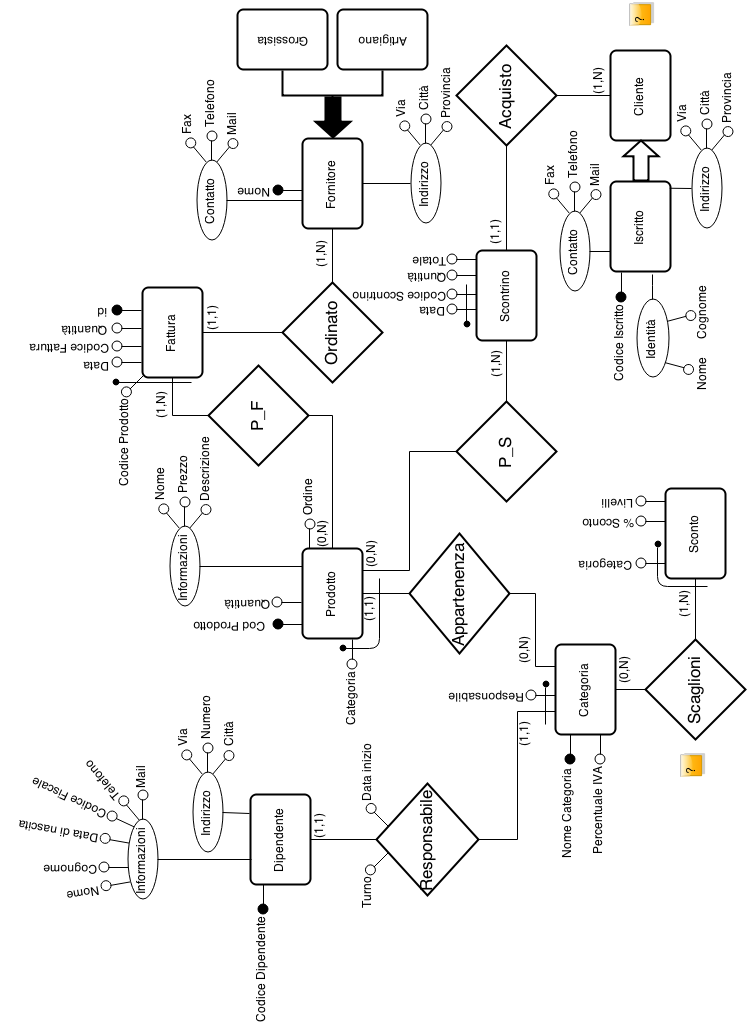
\includegraphics[scale=0.52]{include/progettazioneConcettuale/schemaER/output}
\end{figure}


\section{Progettazione Logica}

\subsubsection{Modello Relazionale}

Seguendo i procedimenti di trasformazione dello schema-ER al modello Relazionale abbiamo ottenuto: \newline
PRODOTTO (\underline{CodProdotto}, Nome, Descrizione, Quantit\`a, Costo, PercentualeIVA, Categoria) \newline
SCONTRINO (\underline{Prodotto}, \underline{Data}, \underline{CodScontrino}, Quantit\`a, Subtotale, Iscritto) \newline
CERTIFICA (\underline{Prodotto}, \underline{Data}, \underline{CodScontrino}) \newline
FATTURA (\underline{Prodotto}, \underline{CodFattura}, Data, Quantit\`a, Fornitore) \newline
REGISTRATO (\underline{Prodotto}, \underline{Codice Fattura}) \newline
CATEGORIA (\underline{Nome Categoria}) \newline
SCONTO (\underline{Categoria}, \underline{Livello}, \underline{PercentualeSconto}, \underline{TettoMax}) \newline
SCAGLIONI (\underline{Categoria}, \underline{Livello}) \newline
ISCRITTO (\underline{CodIscritto}, Nome, Cognome, Fax, Telefono, Mail, Indirizzo) \newline
FORNITORE (\underline{Nome}, Fax, Telefono, Mail, Indirizzo) \newline
DIPENDENTE (\underline{CodDipendente}, Nome, Cognome, Data Nascita, Codice Fiscale, Telefono, Mail, Data Inizio, Categoria) \\

Qui vengono espressi i vincoli non esprimibili nel modello relazionale:
\begin{itemize}
\item In PRODOTTO vincolo d'integrit\`a di categoria con CATEGORIA
\item In SCONTRINO vincolo d'integrit\`a di prodotto con CERTIFICA
\item In SCONTRINO vincolo d'integrit\`a di iscritto con ISCRITTO
\item In CERTIFICA vincolo d'integrit\`a di prodotto con PRODOTTO
\item In CERTIFICA vincolo d'integrit\`a di codice scontrino con SCONTRINO
\item In CERTIFICA vincolo d'integrit\`a di data con SCONTRINO
\item In FATTURA vincolo d'integrit\`a di prodotto con REGISTRATO
\item In FATTURA vincolo d'integrit\`a di fornitore con FORNITORE
\item In REGISTRATO vincolo d'integrit\`a di prodotto con PRODOTTO
\item In REGISTRATO vincolo d'integrit\`a di codice fattura con FATTURA
\item In SCONTO vincolo d'integrit\`a di categoria con SCAGLIONI
\item In SCAGLIONI vincolo d'integrit\`a di categoria con CATEGORIA
\item In SCAGLIONI vincolo d'integrit\`a di livelli con SCONTO
\item In DIPENDENTE vincolo d'integrit\`a di categoria con CATEGORIA \\

\end{itemize}

Inoltre per alcuni attributi abbiamo attribuito le seguenti propriet\`a:
\begin{itemize}
\item In PRODOTTO Descrizione, Foto possono essere NULL
\item In ISCRITTO Fax pu\`o essere NULL
\item In FORNITORE Fax pu\`o essere NULL
\item In DIPENDENTE Mail pu\`o essere NULL
\item In SCONTO il tetto-max pu\`o essere NULL

\end{itemize}


\subsubsection{Create Table}
Prima di creare le tabelle abbiamo inserito le seguenti righe di codice:

\lstinputlisting[language=SQL,firstline=1,lastline=11]{res/code/createtable.sql}
In modo da non incorrere in errori in caso di ricreazione delle tabelle. \newline
I create table veri e propri sono i seguenti:

\lstinputlisting[language=SQL,firstline=13,lastline=15]{res/code/createtable.sql}
crea la tabella Categoria con chiave primaria NomeCategoria;

\lstinputlisting[language=SQL,firstline=16,lastline=27]{res/code/createtable.sql}
crea la tabella Sconto che ha come chiave primaria l'attributo Id;

\lstinputlisting[language=SQL,firstline=28,lastline=36]{res/code/createtable.sql}
Crea la tabella Scaglione (relazione tra Sconto e Categoria), ha come chiave entrambi i suoi campi (Categoria e Sconto) che sono chiave esterna per Categoria e Sconto rispettivamente. Sia Categoria che Sconto hanno il vincolo DELETE ON CASCADE in quanto vogliamo che alla cancellazione di una Categoria anche gli sconti a questa associata vengano cancellati (con l'intervento aggiuntivo del trigger delete\_categoria spiegato successivamente), mentre per l'eliminazione di Sconto deve essere eliminata la tupla corrispondente di Scaglione ma mantenuta la Categoria associata (in quanto potrebbe essere non vuota);

\lstinputlisting[language=SQL,firstline=38,lastline=54]{res/code/createtable.sql}
Crea tabella Dipendente con chiave primaria CodDipendente e Categoria come chiave esterna con vincolo ON DELETE CASCADE in modo tale che all'eliminazione (evento raro ma possibile) di una categoria anche il dipendente venga eliminato;

\lstinputlisting[language=SQL,firstline=56,lastline=67]{res/code/createtable.sql}
crea la tabella Prodotto con chiave primaria CodProdotto e chiave esterna Categoria. In caso di cancellazione di categoria agisce il trigger delete\_categoria che impedisce l'eliminazione in caso di esistenza di prodotti in quella categoria;

\lstinputlisting[language=SQL,firstline=68,lastline=80]{res/code/createtable.sql}
crea la tabella Iscritto con chiave primaria CodIscritto;

\lstinputlisting[language=SQL,firstline=82,lastline=93]{res/code/createtable.sql}
crea la tabella Scontrino con chiave primaria Id e chiave esterna Iscritto a cui viene associato il vincolo ON DELETE CASCADE che alla cancellazione di un iscritto procede alla cancellazione di tutti i suoi scontrini (qui interviene il trigger delete certifica che verr\`a spiegato successivamente). Scontrino si riferisce alle singole righe di uno scontrino, lo scontrino totale viene identificato dal CodScontrino. Abbiamo fatto questa scelta in quanto la maggior parte delle azioni sul database vengono eseguite sulle singole righe e non sullo scontrino totale (questo fatto si ritrova anche nella tabella Fattura);

\lstinputlisting[language=SQL,firstline=95,lastline=102]{res/code/createtable.sql}
crea la tabella Certifica (relazione tra prodotto e scontrino) con chiave primaria Prodotto e Scontrino entrambe anche chiavi esterne per le tabelle Prodotto e Scontrino rispettivamente;

\lstinputlisting[language=SQL,firstline=104,lastline=112]{res/code/createtable.sql}
crea la tabella Fornitore con chiave primaria Nome in quanto univoco;

\lstinputlisting[language=SQL,firstline=114,lastline=123]{res/code/createtable.sql}
crea la tabella Fattura, che si riferisce alle singole righe di fattura, la fattura totale viene identificata dal CodFattura. Abbiamo fatto questa scelta in quanto la maggior parte delle azioni sul database vengono eseguite sulle singole righe e non sulla fattura totale. La chiave primaria \`e Id;

\lstinputlisting[language=SQL,firstline=125,lastline=133]{res/code/createtable.sql}
crea la tabella Registrato (relazione tra Prodotto e Fattura) con chiave primaria Prodotto e Fattura entrambe chiavi esterne per le relazioni Prodotto e Fattura rispettivamente;


\subsubsection{Procedure}

\lstinputlisting[language=SQL,caption=Nuovo Livello]{res/code/Procedura_NuovoLivello.sql}

Questa Procedure esegue diversi controlli:
\begin{enumerate}

\item Controlla la percentuale di sconto inserita sia maggiore di zero

\item Se la categoria collegata al livello di sconto esiste

\item Se non esiste gi\`a lo stesso livello che deve essere aggiunto

\item Controlli sulla scalarit\`a per stessa categoria di riferimento. In particolare controlla se non esistono altri livelli con numero livello pi\`u alto, percentuale sconto pi\`u alto o tetto massimo pi\`u alto; in quanto non avrebbe senso l'inserimento altrimento.
\end{enumerate}

Se queste condizioni sono negate viene generato un errore, altrimenti procede all'inserimento di un nuovo livello di sconto relativo ad una categoria ricevuta come input (la categoria deve esistere a priori).


\section {Implementazione codice}

\subsubsection{Create Table}
Prima di creare le tabelle abbiamo inserito le seguenti righe di codice:

\lstinputlisting[language=SQL,firstline=1,lastline=11]{res/code/createtable.sql}
In modo da non incorrere in errori in caso di ricreazione delle tabelle. \newline
I create table veri e propri sono i seguenti:

\lstinputlisting[language=SQL,firstline=13,lastline=15]{res/code/createtable.sql}
crea la tabella Categoria con chiave primaria NomeCategoria;

\lstinputlisting[language=SQL,firstline=16,lastline=27]{res/code/createtable.sql}
crea la tabella Sconto che ha come chiave primaria l'attributo Id;

\lstinputlisting[language=SQL,firstline=28,lastline=36]{res/code/createtable.sql}
Crea la tabella Scaglione (relazione tra Sconto e Categoria), ha come chiave entrambi i suoi campi (Categoria e Sconto) che sono chiave esterna per Categoria e Sconto rispettivamente. Sia Categoria che Sconto hanno il vincolo DELETE ON CASCADE in quanto vogliamo che alla cancellazione di una Categoria anche gli sconti a questa associata vengano cancellati (con l'intervento aggiuntivo del trigger delete\_categoria spiegato successivamente), mentre per l'eliminazione di Sconto deve essere eliminata la tupla corrispondente di Scaglione ma mantenuta la Categoria associata (in quanto potrebbe essere non vuota);

\lstinputlisting[language=SQL,firstline=38,lastline=54]{res/code/createtable.sql}
Crea tabella Dipendente con chiave primaria CodDipendente e Categoria come chiave esterna con vincolo ON DELETE CASCADE in modo tale che all'eliminazione (evento raro ma possibile) di una categoria anche il dipendente venga eliminato;

\lstinputlisting[language=SQL,firstline=56,lastline=67]{res/code/createtable.sql}
crea la tabella Prodotto con chiave primaria CodProdotto e chiave esterna Categoria. In caso di cancellazione di categoria agisce il trigger delete\_categoria che impedisce l'eliminazione in caso di esistenza di prodotti in quella categoria;

\lstinputlisting[language=SQL,firstline=68,lastline=80]{res/code/createtable.sql}
crea la tabella Iscritto con chiave primaria CodIscritto;

\lstinputlisting[language=SQL,firstline=82,lastline=93]{res/code/createtable.sql}
crea la tabella Scontrino con chiave primaria Id e chiave esterna Iscritto a cui viene associato il vincolo ON DELETE CASCADE che alla cancellazione di un iscritto procede alla cancellazione di tutti i suoi scontrini (qui interviene il trigger delete certifica che verr\`a spiegato successivamente). Scontrino si riferisce alle singole righe di uno scontrino, lo scontrino totale viene identificato dal CodScontrino. Abbiamo fatto questa scelta in quanto la maggior parte delle azioni sul database vengono eseguite sulle singole righe e non sullo scontrino totale (questo fatto si ritrova anche nella tabella Fattura);

\lstinputlisting[language=SQL,firstline=95,lastline=102]{res/code/createtable.sql}
crea la tabella Certifica (relazione tra prodotto e scontrino) con chiave primaria Prodotto e Scontrino entrambe anche chiavi esterne per le tabelle Prodotto e Scontrino rispettivamente;

\lstinputlisting[language=SQL,firstline=104,lastline=112]{res/code/createtable.sql}
crea la tabella Fornitore con chiave primaria Nome in quanto univoco;

\lstinputlisting[language=SQL,firstline=114,lastline=123]{res/code/createtable.sql}
crea la tabella Fattura, che si riferisce alle singole righe di fattura, la fattura totale viene identificata dal CodFattura. Abbiamo fatto questa scelta in quanto la maggior parte delle azioni sul database vengono eseguite sulle singole righe e non sulla fattura totale. La chiave primaria \`e Id;

\lstinputlisting[language=SQL,firstline=125,lastline=133]{res/code/createtable.sql}
crea la tabella Registrato (relazione tra Prodotto e Fattura) con chiave primaria Prodotto e Fattura entrambe chiavi esterne per le relazioni Prodotto e Fattura rispettivamente;


\subsubsection{Procedure}

\lstinputlisting[language=SQL,caption=Nuovo Livello]{res/code/Procedura_NuovoLivello.sql}

Questa Procedure esegue diversi controlli:
\begin{enumerate}

\item Controlla la percentuale di sconto inserita sia maggiore di zero

\item Se la categoria collegata al livello di sconto esiste

\item Se non esiste gi\`a lo stesso livello che deve essere aggiunto

\item Controlli sulla scalarit\`a per stessa categoria di riferimento. In particolare controlla se non esistono altri livelli con numero livello pi\`u alto, percentuale sconto pi\`u alto o tetto massimo pi\`u alto; in quanto non avrebbe senso l'inserimento altrimento.
\end{enumerate}

Se queste condizioni sono negate viene generato un errore, altrimenti procede all'inserimento di un nuovo livello di sconto relativo ad una categoria ricevuta come input (la categoria deve esistere a priori).

\newpage
\subsubsection{Query}

\paragraph*{Query 1}
Prodotto pi\`u venduto (nota per visualizzare il risultato di questa query abbiamo omesso il campo descrizione)

\begin{verbatim}

+-------------+------------+--------+----------------+------------+-------------+
| CodProdotto | Nome       | Costo  | PercentualeIVA | Categoria  | Num_venduti |
+-------------+------------+--------+----------------+------------+-------------+
|           5 | padella    |  40.00 |             22 | Pentolame  |           5 |
|           6 | padella    |  34.50 |             22 | Pentolame  |           1 |
|          11 | Set. Tazze | 250.00 |             22 | Porcellane |           1 |
|          12 | tovaglia   |  10.00 |             22 | Tovaglie   |           2 |
|          14 | confetti   |   0.10 |             10 | ListeNozze |           1 |
|          15 | teglia     |  39.00 |             22 | Pentolame  |           1 |
|          16 | pentola    |  30.00 |             22 | Pentolame  |           2 |
+-------------+------------+--------+----------------+------------+-------------+

\end{verbatim}

\lstinputlisting[language=SQL,firstline=3,lastline=20,caption=Query 1]{res/code/query.sql}


\paragraph*{Query 2}
Prodotti invenduti

\begin{verbatim}

+-------------+
| CodProdotto |
+-------------+
|           1 |
|           2 |
|           3 |
|           4 |
|           7 |
|           8 |
|           9 |
|          10 |
|          13 |
+-------------+

\end{verbatim}

\lstinputlisting[language=SQL,firstline=25,lastline=28,caption=Query 2]{res/code/query.sql}

\paragraph*{Query 3}
Prodotti acquistati da un certo utente iscritto (per una migliore visualizzazione del risultato abbiamo omesso il campo Descrizione)

\begin{verbatim}

+-------------+------------+--------+----------------+------------+
| CodProdotto | Nome       | Costo  | PercentualeIVA | Categoria  |
+-------------+------------+--------+----------------+------------+
|           5 | padella    |  40.00 |             22 | Pentolame  |
|           5 | padella    |  40.00 |             22 | Pentolame  |
|           5 | padella    |  40.00 |             22 | Pentolame  |
|           5 | padella    |  40.00 |             22 | Pentolame  |
|           5 | padella    |  40.00 |             22 | Pentolame  |
|           6 | padella    |  34.50 |             22 | Pentolame  |
|          11 | Set. Tazze | 250.00 |             22 | Porcellane |
|          12 | tovaglia   |  10.00 |             22 | Tovaglie   |
|          14 | confetti   |   0.10 |             10 | ListeNozze |
|          16 | pentola    |  30.00 |             22 | Pentolame  |
|          15 | teglia     |  39.00 |             22 | Pentolame  |
|          16 | pentola    |  30.00 |             22 | Pentolame  |
+-------------+------------+--------+----------------+------------+

\end{verbatim}

\lstinputlisting[language=SQL,firstline=38,lastline=41,caption=Query 3]{res/code/query.sql}

\paragraph*{Query 4}
Fornitore da cui ho comprato di pi\`u (per una migliore visualizzazione del risultato abbiamo omesso il campo Fax e Telefono)

\begin{verbatim}

+----------+--------------------------+--------------------------+------------------------+
| Nome     |Mail                      | Indirizzo                | Numero_acquisto        |
+----------+--------------------------+--------------------------+------------------------+
| Arzenton |arzenton.scatole@gmail.com| via roma, 51 verona Vr   | 3                      |
+----------+--------------------------+--------------------------+------------------------+

\end{verbatim}

\lstinputlisting[language=SQL,firstline=45,lastline=55,caption=Query 4]{res/code/query.sql}

\paragraph*{Query 5}
Categoria che ha venduto pi\`u prodotti

\begin{verbatim}

+-----------+--------------+
| Categoria | Guadagno_Max |
+-----------+--------------+
| Pentolame |       511.00 |
+-----------+--------------+

\end{verbatim}

\lstinputlisting[language=SQL,firstline=59,lastline=70,caption=Query 5]{res/code/query.sql}

\paragraph*{Query 6}
Iscritti che non hanno mai comprato prodotti da una certa categoria (per una migliore visualizzazione del risultato abbiamo omesso il campo Fax e Telefono) 

\begin{verbatim}

+-------------+------------+-----------+---------------------------+---------------------------+
| CodIscritto | Nome       | Cognome   |Mail                       | Indirizzo                 |
+-------------+------------+-----------+---------------------------+---------------------------+
|           1 | Alessandro | Bari      |alessandro.bari@gmail.com  | Via roma, 10 Verona Vr    |
|           2 | Carlo      | Sindaco   |carlo.sin@gmail.com        | Via S.paolo, 12 Verona Vr |
|           3 | Giovanni   | Mucciacia |giovanni.mu@gmail.com      | Via augusto, 12 Verona Vr |
+-------------+------------+-----------+------------+--------------+---------------------------+

\end{verbatim}

\lstinputlisting[language=SQL,firstline=75,lastline=82,caption=Query 6]{res/code/query.sql}

\newpage
\paragraph*{Query 7}
Giorno della settimana dove vi \`e stato il maggior guadagno

\begin{verbatim}

+------------+-------------+
| Data       | Tot_vendite |
+------------+-------------+
| 2015-01-06 |      381.00 |
+------------+-------------+

\end{verbatim}

\lstinputlisting[language=SQL,firstline=86,lastline=90,caption=Query 7]{res/code/query.sql}

\paragraph*{Query 8}
Nome dipendente responsabile della categoria che ha stampato il maggior numero di scontrini

\begin{verbatim}

+----------+---------------+---------------+
| Nome     | Num_Scontrini | NomeCategoria |
+----------+---------------+---------------+
| Giovanni |             9 | Pentolame     |
+----------+---------------+---------------+

\end{verbatim}

\lstinputlisting[language=SQL,firstline=94,lastline=108,caption=Query 8]{res/code/query.sql}

\paragraph*{Query 9}
Per ogni iscritto il livello di sconto piu alto nella categoria che ha venduto di pi\`u questo mese

\begin{verbatim}

+-------------+------------+---------+-----------------+
| CodIscritto | Nome       | Cognome | Livello_massimo |
+-------------+------------+---------+-----------------+
|           1 | Alessandro | Bari    |               1 |
+-------------+------------+---------+-----------------+

\end{verbatim}

\lstinputlisting[language=SQL,firstline=112,lastline=140,caption=Query 9]{res/code/query.sql}

\newpage
\paragraph*{Query 10}
Per iscritto i suoi scontrini (numero di acquisti) e i livelli (attualmente raggiunti) per ogni categoria.
Nell'esempio visualizziamo gli scontrino dell'utente $1$.

\begin{verbatim}

+-----------------+---------------+-----------------+
| Numero_Acquisti | NomeCategoria | Livello_attuale |
+-----------------+---------------+-----------------+
|               2 | ListeNozze    |               1 |
|              18 | Pentolame     |               1 |
|               2 | Porcellane    |               1 |
|               2 | Tovaglie      |               1 |
+-----------------+---------------+-----------------+

\end{verbatim}

\lstinputlisting[language=SQL,firstline=144,lastline=161,caption=Query 10]{res/code/query.sql}

\subsubsection{Codice PHP}

\`E stata inserita la parte PHP che si occupa di inserire una nuova fattura, inserendo anche, nel caso di un nuovo prodotto, il nuovo prodotto con tutti i suoi campi.


\lstinputlisting[language=PHP,caption=addInvoice.php]{res/code/addInvoice.php}



\end{document}
